\section{Textual Analysis}

All the code used to compute the results shown in the next sections can be seen in the Jupyter notebook \href{https://github.com/mhetacc/crossdem/blob/8645cc832df6ead9163506777cc995e2d70f5bd1/notebooks/text_analysis.ipynb}{mhetacc/crossdem/notebooks/text\_analysis.ipynb}.


\subsection{Token Count and Textual Complexity}

The collected corpus contains 473 speeches from De Gasperi and 72 from Meloni, with a total token count of $609,142$ for De Gasperi and $120,116$ for Meloni.
On average, Meloni's corpus has 1668 tokens per speech, while De Gasperi's has 1287 tokens per speech. Word metrics are shown in table \ref{tab:politician_tokens}.
The text was tokenized with spaCy's Italian model \textit{"it\_core\_news\_sm"}.

I then measured the textual lexical diversity using \textit{MTLD}, which I preferred over the more common \textit{TTR} (Type-Token Ratio) since MTLD is agnostic to corpus size. I used the \textit{LexicalRichness} library\footnote{LexicalRichness is a small Python module to compute textual lexical richness measures: \url{https://pypi.org/project/lexicalrichness/}.} to compute the MTLD for each speech, and then both the average and the median MTLD for both PMs. Results can be seen in table \ref{tab:politician_mtld}.

To better visualize the difference in textual diversity, I plotted the MTLD values of 70 different speeches of Meloni and De Gasperi against each other. The plot can be seen in figure \ref{fig:mtl_comparison}.


\begin{table}[h]
    \centering
    \caption{Total tokens and average tokens per speech for De Gasperi and Meloni.}
    \label{tab:politician_tokens}
    \begin{tabular}{lccc}
        \toprule
        \textbf{Politician} & \textbf{Total Tokens} & \textbf{Speeches Count} & \textbf{Avg Tokens/Speech} \\
        \midrule
        De Gasperi           & 609,142               & 473                   & 1,287.83                   \\
        Meloni              & 120,116               & 72                    & 1,668.28                   \\
        \bottomrule
    \end{tabular}
\end{table}


\begin{table}[h]
    \centering
    \caption{MTLD metrics for De Gasperi and Meloni.}
    \label{tab:politician_mtld}
    \begin{tabular}{lcc}
        \toprule
        \textbf{Politician} & \textbf{Avg MTLD} & \textbf{Median MTLD} \\
        \midrule
        De Gasperi           & 141.830           & 137.642              \\
        Meloni              & 106.745           & 104.918              \\
        \bottomrule
    \end{tabular}
\end{table}


\begin{figure}[h]
  \centering
  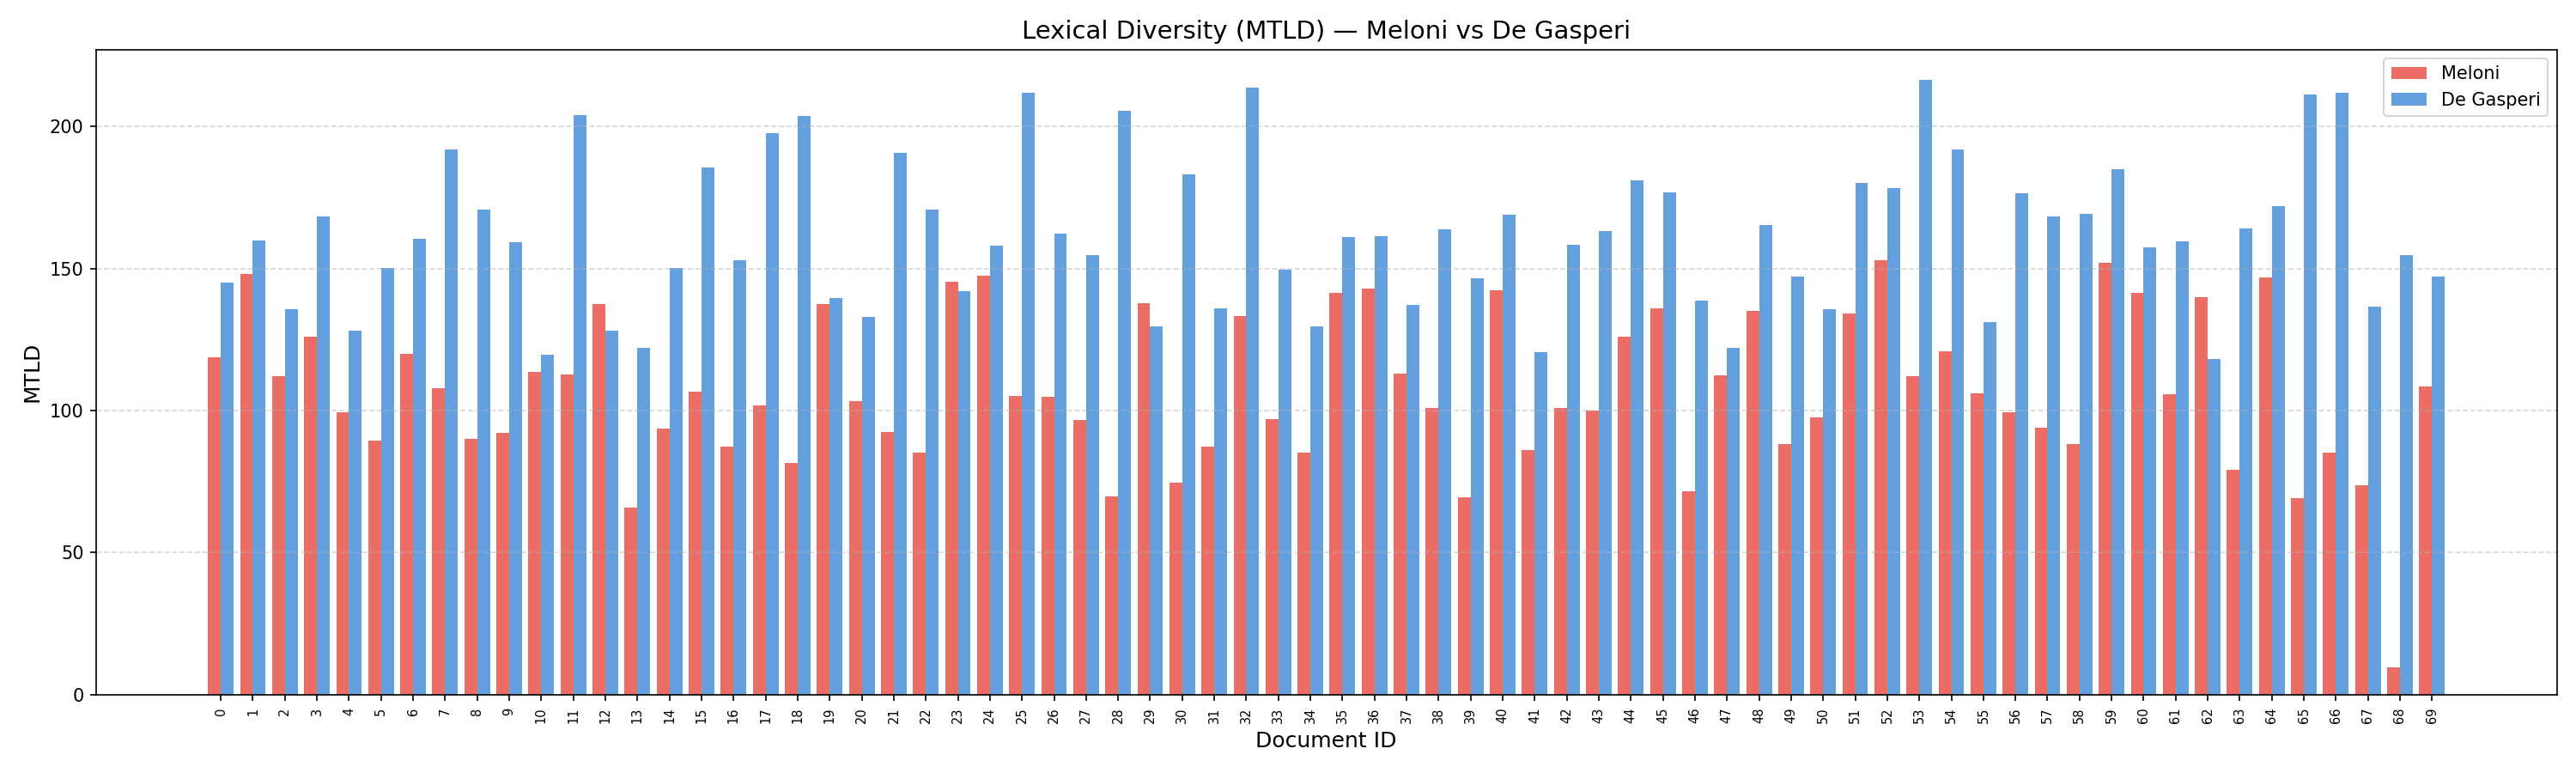
\includegraphics[width=\linewidth]{images/mtld_comparison.png}
  \caption{MTLD values for 60 different speeches (30 for each Prime Minister), randomly sampled. On the Y-axis the MTLD values are reported, while on the X-axis there are the relative IDs for the pairs of speeches. Each pair of speeches is represented by a two vertical bars (one red for Meloni, one blue for De Gasperi). Bar height represents their respective speech's MTLD value. The medians for both Prime Ministers are shown by the two horizontal dotted lines.}
  \label{fig:mtl_comparison}
\end{figure}


\subsection{Vocabulary Comparison}

I then wanted to see differences and similarities in the two Prime Ministers' vocabulary. I thus extracted from the corpus a filtered subset of tokens (example in listing \ref{code:extract_tokens}), then I used the \textit{Counter} method from the \textit{collections} library to count the 1000 most commonly used words for both PMs.

Of the top-1000 words, 487 are in common, with a Jaccard similarity of $32.19\%$.

After extracting the top-1000 words by usage frequency for each PM, I cross-compared them. The results are shown in table \ref{tab:word_comparison_aligned}. The first column shows words that are in common, whose compound frequency ($meloni\_freq[word]+degasperi\_freq[word]$) is highest. The second column shows words that are only found in De Gasperi's corpus (Meloni's frequency for those words is zero). The third column shows words that are only found in Meloni's corpus (De Gasperi's frequency for those words is zero).

It is interesting to see that words in common are about transversal themes, such as \textit{italia}, \textit{popolo}, \textit{libertà}, and \textit{democrazia}. Interestingly, \textit{europa} is a top-20 shared word, showing us that the theme was and still is relevant even though the two PMs were born almost 100 years apart from each other.

On the other hand, the PM-specific words show us how the public discourse changes in the different periods: there are some themes that seem to have disappeared; for example, in the De Gasperi-only top 20 we see words such as \textit{comunismo}, \textit{socialisti}, and \textit{marshall}, all of which were extremely relevant 70 years ago.
In the Meloni-only top 20 we find words that simply could not have mattered back then, even though today they are absolutely central, such as \textit{trump}, \textit{ucraina}, \textit{putin}, and \textit{hamas}.

We can also see some examples of how the language itself changes over time: De Gasperi used quite often the word \textit{dinanzi}, while Meloni often uses \textit{dopodiché}. Both of these words are never used by the other Prime Minister.

To try to visualize how close (or far apart) the two PM's vocabularies are, I visualized their top-1000 words in a t-SNE scatter plot using the \textit{scikit-learn} library. The results (in figure \ref{fig:visual_top1k}) show us that, with the exception of the words in common (in purple), the two vocabularies seem to be quite far apart, clustering in different regions.


\begin{lstlisting}[language={python},label={code:extract_tokens}, caption={Extract and filter words with tokenize function.}]
def tokenize(text):
    return [token.text.lower() for token in nlp(text)
            if token.is_alpha       # only alphanumeric
            and not token.is_stop   # no stop-words
            and len(token)>3        # removes articles and some filler words
            ]
\end{lstlisting}


\begin{table}[h]
    \centering
    \caption{Comparison of most frequent words common to both PM. Last two columns show words specific to only one PM.}
    \label{tab:word_comparison_aligned}
    \begin{tabular}{clll}
        \toprule
        \textbf{Rank} & \textbf{Common Words \hfill (Sum)} & \textbf{De Gasperi Only \hfill (Freq)} & \textbf{Meloni Only \hfill (Freq)} \\
        \midrule
        1  & italia \hfill (1967)     & gasperi \hfill (458)    & euro \hfill (88)           \\
        2  & popolo \hfill (1201)     & comunisti \hfill (412)  & ucraina \hfill (85)        \\
        3  & libertà \hfill (1071)    & trieste \hfill (309)    & sottotitoli \hfill (65)    \\
        4  & guerra \hfill (927)      & comunista \hfill (241)  & dopodiché \hfill (48)      \\
        5  & politica \hfill (912)    & avvenire \hfill (237)   & trump \hfill (46)          \\
        6  & pace \hfill (910)        & togliatti \hfill (207)  & infrastrutture \hfill (37) \\
        7  & italiano \hfill (828)    & trento \hfill (173)     & approccio \hfill (32)      \\
        8  & presidente \hfill (733)  & comunismo \hfill (171)  & competitività \hfill (30)  \\
        9  & democrazia \hfill (708)  & socialisti \hfill (170) & gaza \hfill (28)           \\
        10 & partito \hfill (682)     & oratore \hfill (165)    & migrazione \hfill (28)     \\
        11 & bisogna \hfill (661)     & deputati \hfill (158)   & scenario \hfill (26)       \\
        12 & italiani \hfill (605)    & trentino \hfill (149)   & centrodestra \hfill (26)   \\
        13 & soprattutto \hfill (567) & dittatura \hfill (145)  & record \hfill (23)         \\
        14 & europa \hfill (563)      & democratici \hfill (143) & hamas \hfill (23)          \\
        15 & sociale \hfill (548)     & nenni \hfill (142)      & palestina \hfill (20)      \\
        16 & cioè \hfill (535)        & voti \hfill (137)       & meloni \hfill (19)         \\
        17 & altra \hfill (530)       & degasperi \hfill (127)  & food \hfill (19)           \\
        18 & amici \hfill (522)       & onorevole \hfill (126)  & mattoni \hfill (19)        \\
        19 & nazione \hfill (508)     & dinanzi \hfill (125)    & buongiorno \hfill (19)     \\
        20 & senso \hfill (502)       & marshall \hfill (122)   & putin \hfill (19)          \\
        \bottomrule
    \end{tabular}
\end{table}


\begin{figure}[h]
  \centering
  \includegraphics[width=\linewidth]{images/tsne_melonidegasperi.png}
  \caption{t-SNE projection of the top-1000 most frequent words for each Prime Minister, converted into vector embeddings and plotted in a two-dimensional space. Red points represent words exclusive to Meloni, blue points words exclusive to De Gasperi, and purple points words shared by both}
  \label{fig:visual_top1k}
\end{figure}


\subsection{Limitations}

A better filtering of the extracted words would be needed: for example, "gasperi" and "degasperi" should ideally be merged into the bigram "de gasperi", if not removed entirely, since he did not refer to himself in the third person.

This could be achieved by applying named entity recognition (NER) to identify and merge multi-word names, or by post-processing the token list to combine frequent bigrams corresponding to named entities.

Additionally, a custom stop-word list could be compiled: for example, in Meloni's corpus the word "sottotitoli" appears often, but was likely added in post-production by the video uploader.